\documentclass[crop]{standalone}
\usepackage[usenames,dvipsnames,svgnames]{xcolor}
\usepackage{tikz}
\usetikzlibrary{arrows,shapes} % tikz package already loaded by 'tikz' option
\makeatletter
\begin{document}
\newcommand{\dred}    [1]	{\textcolor{BrickRed!60!Red}{#1}}
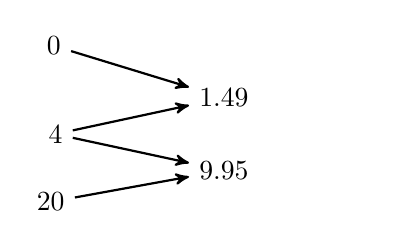
\begin{tikzpicture}[->,>=stealth',node distance=1.5cm, thick]
	\node (A) {};
	\node (B)	[above left of=A,yshift=-.6cm,xshift=-.7cm] 	{$1.49$};
	\node (A2) 	[left of=A] 									{};
	\node (A3) 	[left of=A2,xshift=-.9cm] 						{$4$};
	\node (B2)	[above left of=B,yshift=-.4cm,xshift=-1.1cm]	{$0$};
	\node (C) 	[below left of=A,yshift=+.6cm,xshift=-.7cm] 	{\dred{$9.95$}};
	\node (C2)	[left of=C,yshift=-.4cm,xshift=-.7cm]			{$20$};
	\path
	%	(B) edge	(A)
	%(C) edge	(A)
	(B2) edge	(B)
	(A3) edge	(B)
	(A3) edge	(C)
	(C2) edge	(C)
	;
\end{tikzpicture}


\end{document}
